\subsection{Overview}
\begin{frame}
    \frametitle{Introduction to OllyDbg}
    \begin{itemize}
        \item Freeware
        \item Contains a lot of \emph{cracker friendly} features
        \item Pluggable through a multitude of languages
        \item Scriptable through OllyScript
        \item Contains a powerful disassembler
            \pedbullet{Also available as a library}
    \end{itemize}
\end{frame}

\begin{frame}
    \frametitle{Learning Curve}
    \begin{itemize}
        \item Very daunting on first launch
        \item There are tons of \emph{hidden} features
            \pedbullet{I am still finding new ones}
        \item Fortunately there is excellent documentation
        \item The best way to learn however ...
            \begin{itemize}
                \item Open something in OllyDbg
                \item Play around with the various features
                \item Explore the various windows
                \item Customize your environment with the features you will be using
            \end{itemize}
    \end{itemize}
\end{frame}

\subsection{Overview of Views}
\begin{frame}
    \frametitle{CPU Main Window}
    \begin{center}
        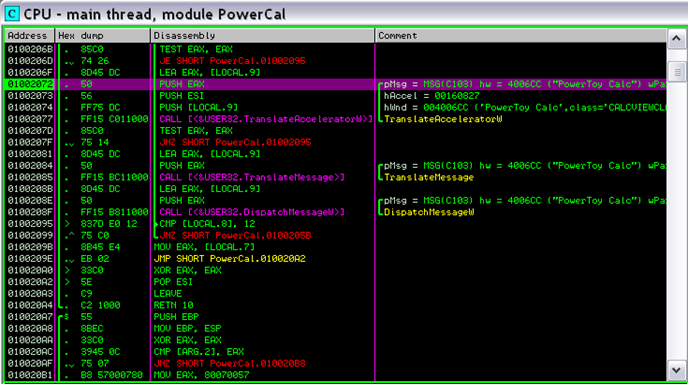
\includegraphics[scale=.75]{images/olly/cpu.png} \\
    \end{center}
    \begin{itemize}
        \item Comment-able disassembly
        \item Argument enumeration
        \item Smart de-referencing
    \end{itemize}
\end{frame}

\begin{frame}
    \frametitle{CPU Registers}
    \begin{columns}[T]
        \column{.5\textwidth}
            \begin{itemize}
                \item Editable register values
                \item CPU flags
                \item Smart de-referencing
                \item Floating point, MMX, 3DNow! Support
                \item Follow in stack/dump shortcuts
            \end{itemize}
        \column{.5\textwidth}
            \begin{center}
                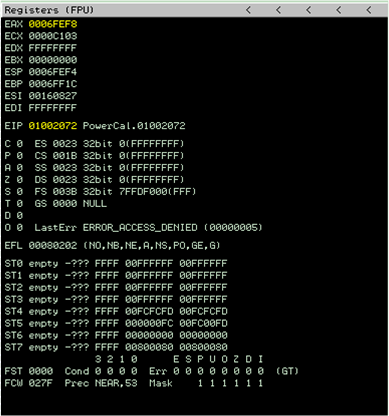
\includegraphics[scale=.45]{images/olly/cpu_registers.png}
            \end{center}
    \end{columns}
\end{frame}

\begin{frame}
    \frametitle{CPU Stack}
    \begin{columns}[T]
        \column{.5\textwidth}
            \begin{itemize}
                \item Editable
                \item Lockable
                \item View relative to ESP/EBP
                \item Smart de-referencing
                \item SEH chain
                \item Saved frames
                \item ASCII/Unicode dump
            \end{itemize}
        \column{.5\textwidth}
            \begin{center}
                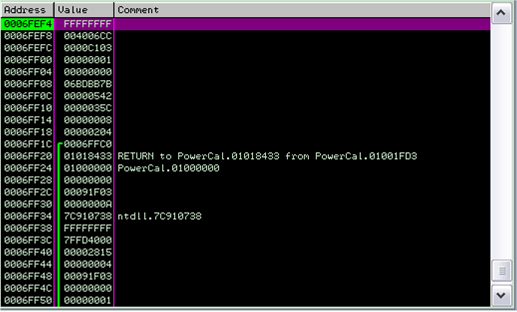
\includegraphics[scale=.60]{images/olly/cpu_stack.png}
            \end{center}
    \end{columns}
\end{frame}

\begin{frame}
    \frametitle{CPU Dump}
    \begin{columns}[T]
        \column{.5\textwidth}
            \begin{itemize}
                \item Unique and handy OllyDbg feature
                \item Multiple view types: hex, text, disassembly, long pointers, PE header and it's extensible with plug-ins (see SPECFUNC)
            \end{itemize}
        \column{.5\textwidth}
            \begin{center}
                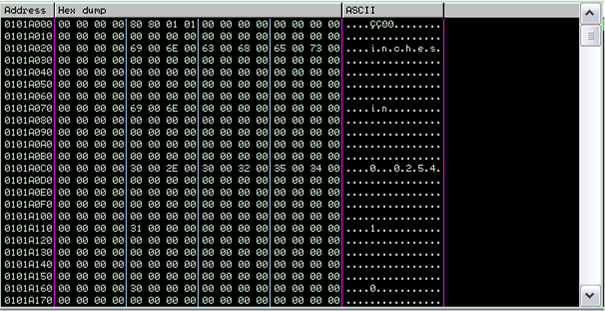
\includegraphics[scale=.60]{images/olly/cpu_dump.png}
            \end{center}
    \end{columns}
\end{frame}

\begin{frame}
    \frametitle{Log Window}
    \begin{center}
        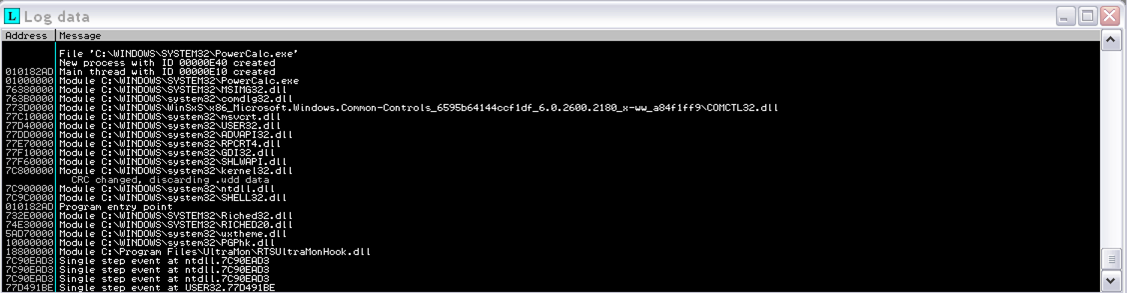
\includegraphics[scale=.60]{images/olly/log.png} \\
    \end{center}
    \begin{itemize}
        \item Debugger / plug-in output messages
            \pedbullet{Breakpoint / log breakpoint output}
            \pedbullet{Access violations}
            \pedbullet{Etc...}
        \item Debuggee messages through OutputDebugString() API
    \end{itemize}
\end{frame}

\begin{frame}
    \frametitle{Call Stack}
    \begin{center}
        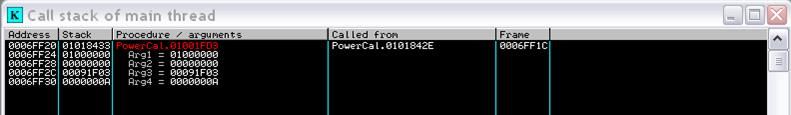
\includegraphics[scale=.50]{images/olly/call_stack.png} \\
    \end{center}
    \begin{itemize}
        \item Collapsible with arguments
        \item Stack walking is not an exact science, especially when standard EBP based frames are not used.
        \item Olly is pretty smart about it
    \end{itemize}
\end{frame}

\begin{frame}
    \frametitle{Threads}
    \begin{center}
        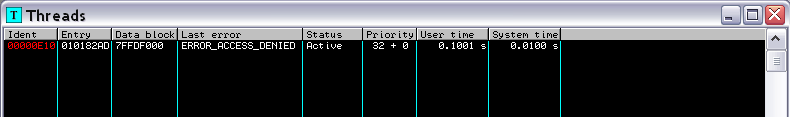
\includegraphics[scale=.75]{images/olly/threads.png} \\
    \end{center}
    \begin{itemize}
        \item List of threads in current process
    \end{itemize}
    \begin{uncoverenv}
        \tip{When attempting to determine which thread processes an input, say for example network packets, fire off some packets forcing the process to work and watch the User/System time columns.}
    \end{uncoverenv}
\end{frame}

\begin{frame}
    \frametitle{Executable Modules}
    \begin{center}
        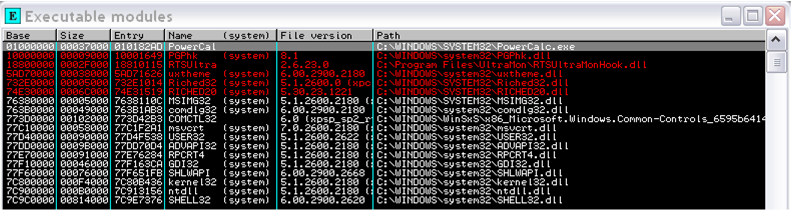
\includegraphics[scale=.60]{images/olly/executable_modules.png} \\
    \end{center}
    \begin{itemize}
        \item List of modules currently loaded in the debuggee's process space
        \item The Name column contains the �hidden� system tag (run traces)
        \item Ctrl+N to view exported names
        \item Breakpoints / log breakpoints can be set
        \item Olly knows the argument types for a lot of standard API calls
    \end{itemize}
\end{frame}

\begin{frame}
    \frametitle{Memory Map}
    \begin{columns}[T]
        \column{.5\textwidth}
            \begin{itemize}
                \item Searchable full-range memory map
                \item Stack is tagged, heaps are not
                \item OllyDbg Heap Vis plug-in allows you to list, search and visualize the heap
            \end{itemize}
        \column{.5\textwidth}
            \begin{center}
                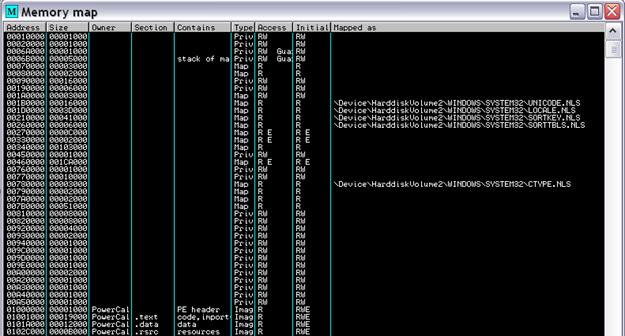
\includegraphics[scale=.60]{images/olly/memory_map.png}
            \end{center}
    \end{columns}
\end{frame}

\begin{frame}
    \frametitle{Breakpoints}
    \begin{center}
        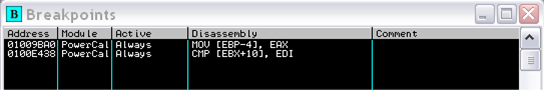
\includegraphics[scale=.50]{images/olly/breakpoints.png} \\
    \end{center}
    \begin{itemize}
        \item OllyDbg supports regular breakpoints, conditional breakpoints and conditional log breakpoints
        \item Breakpoints set in the main module are persistent across debugger sessions.
        \item OllyDbg BP Manager plug-in allows you to import/export breakpoints lists
        \item You can use the BP Manager to automatically load breakpoints on module load
    \end{itemize}
\end{frame}

\begin{frame}
    \frametitle{Bookmarks}
    \begin{center}
        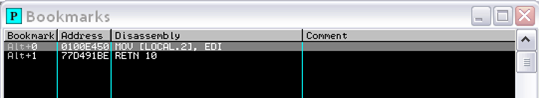
\includegraphics[scale=.50]{images/olly/bookmarks.png} \\
    \end{center}
    \begin{itemize}
        \item Bookmarking is provided by a plug-in bundled with OllyDbg
        \item Simply set and quick jump to various locations
        \item Identical to "marks" in IDA
    \end{itemize}
\end{frame}

\begin{frame}
    \frametitle{SEH Chain}
    \begin{columns}[T]
        \column{.5\textwidth}
            \begin{itemize}
                \item Unique OllyDbg feature
                \item Does not show the vector based exception handling chain
            \end{itemize}
        \column{.5\textwidth}
            \begin{center}
                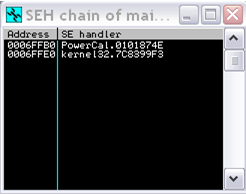
\includegraphics[scale=.50]{images/olly/seh_chain.png}
            \end{center}
    \end{columns}
\end{frame}

\begin{frame}
    \frametitle{Watch Expressions}
    \begin{columns}[T]
        \column{.5\textwidth}
            \begin{itemize}
                \item OllyDbg supports an expression language allowing the user to create real-time watches
                \item Useful when tracking changes to complex data types
            \end{itemize}
        \column{.5\textwidth}
            \begin{center}
                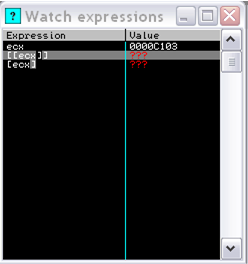
\includegraphics[scale=.50]{images/olly/watch_expressions.png}
            \end{center}
    \end{columns}
\end{frame}

\begin{frame}
    \frametitle{Handles}
    \begin{center}
        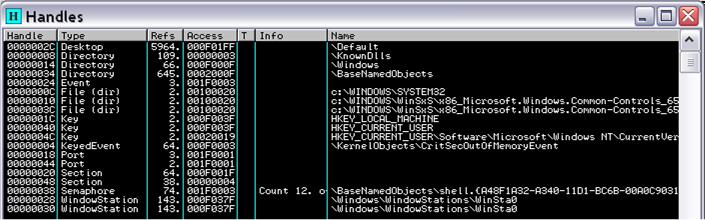
\includegraphics[scale=.50]{images/olly/handles.png} \\
    \end{center}
    \begin{itemize}
        \item List of open handles
        \item Tag / untag
            \pedbullet{Not sure entirely what this is for.}
    \end{itemize}
\end{frame}

\begin{frame}
    \frametitle{Plug-ins}
    \begin{block}{Fact}
    OllyDbg has excellent plug-in support and great API documentation. Much better than IDA.
    \end{block}
    \begin{itemize}
        \item GODUP
            \pedbullet{Load labels and comments from IDA}
        \item OllyDump
            \pedbullet{Dump the running process to disk, IAT rebuilding (malware purposes)}
        \item Heap Vis
            \pedbullet{Enumerate and search process heap}
        \item Breakpoint Manager
            \pedbullet{Import / export breakpoint sets}
        \item De-Attach Helper
            \pedbullet{Adds detach support and WinDbg similar "attach to last" functionality}
    \end{itemize}
\end{frame}


\subsection{Driving OllyDbg}
\begin{frame}
    \frametitle{Hot Keys}
    \begin{center}
        \begin{tabular}{l l}
            \uncover{\cellcolor{lightblue} F9         & \cellcolor{lightblue}Execute debuggee         \\}
            \uncover{                      CTRL + F9  & Execute until return                          \\}
            \uncover{\cellcolor{lightblue} ALT + F9   & \cellcolor{lightblue}Execute until user code  \\}
            \uncover{                      F12        & Pause                                         \\}
            \uncover{\cellcolor{lightblue} F7         & \cellcolor{lightblue}Step into                \\}
            \uncover{                      F8         & Step over                                     \\}
            \uncover{\cellcolor{lightblue} F2         & \cellcolor{lightblue}Set / clear breakpoint   \\}
            \uncover{                      CTRL + G   & Follow expression                             \\}
            \uncover{\cellcolor{lightblue} any key    & \cellcolor{lightblue}Add comment              \\}
            \uncover{                      :          & Add label                                     \\}
        \end{tabular}
    \end{center}
\end{frame}

\begin{frame}
    \frametitle{Following Expressions}
    \begin{center}
        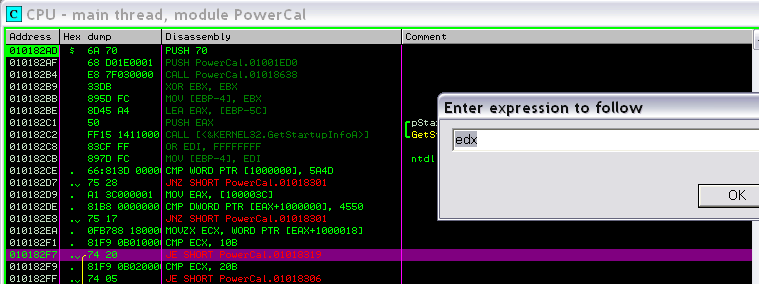
\includegraphics[scale=.25]{images/olly/follow_expression.png} \\
    \end{center}
    \begin{itemize}
        \item Use CTRL+G to open the \emph{follow expression} window
        \item You can specify an address, register, or the label of a function, such as recv or sprintf
    \end{itemize}
    \begin{uncoverenv}
        \tip{Sometimes you have to CTRL+G \alert{twice} in order to get it to resolve to the actual location. This appears to be a bug.}
    \end{uncoverenv}
\end{frame}

\begin{frame}
    \frametitle{Software Breakpoints}
    \begin{center}
        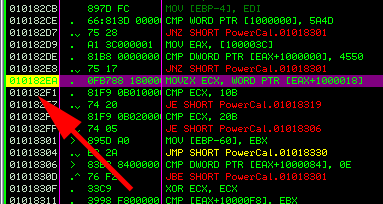
\includegraphics[scale=.50]{images/olly/set_breakpoint.png} \\
    \end{center}
    \begin{itemize}
        \item Set focus on the target instruction
        \item Hit F2 to set / unset the breakpoint
    \end{itemize}
\end{frame}

\begin{frame}
    \frametitle{Hardware Breakpoints}
    \begin{center}
        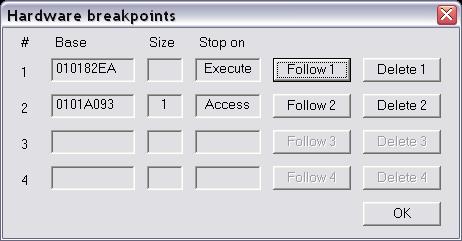
\includegraphics[scale=.30]{images/olly/hardware_breakpoints.png} \\
    \end{center}
    \begin{itemize}
        \item You get 4 hardware breakpoints
        \item CPU supported, so transparent to software
        \item Set focus on the target instruction or memory address
        \item Right click $\rightarrow$ breakpoint $\rightarrow$ hardware
        \item Three classes: access, write and execute
        \item Three sizes: byte (1), word (2), dword (4)
    \end{itemize}
\end{frame}

\begin{frame}
    \frametitle{Memory Breakpoints}
    \begin{itemize}
        \item Actually it's just memory \alert{breakpoint}, you get one
        \item OllyDbg accomplishes this task by changing the permissions of the page that contains your target address
        \item You should opt to use hardware breakpoints over this feature
        \item In case you really need a 5th on-access type breakpoint, it's there for you
    \end{itemize}
\end{frame}

\begin{frame}
    \frametitle{Enumerating Functions}
    \begin{center}
        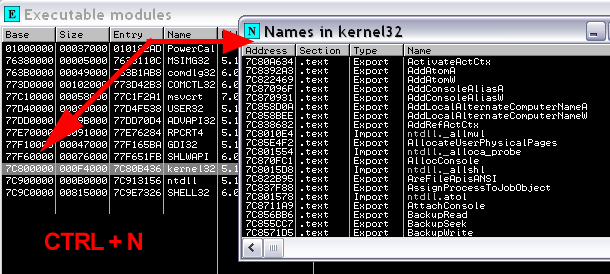
\includegraphics[scale=.40]{images/olly/enumerate_functions.png} \\
    \end{center}
    \begin{itemize}
        \item Go to the \emph{executable modules} window
        \item Highlight the DLL you are interested in
        \item Hit \alert{CTRL + N} to pull up a list of imports/exports
        \item You can hit F2 directly on this list to set breakpoints
    \end{itemize}
\end{frame}

\begin{frame}
    \frametitle{Searching}
    \begin{columns}[T]
        \column{.6\textwidth}
            \begin{itemize}
                \item One of the best OllyDbg features
                \item You can search modules, memory, stack
                \item Search for strings or commands
                \item Search for variable register commands
                \item Search for all string references
            \end{itemize}
        \column{.4\textwidth}
            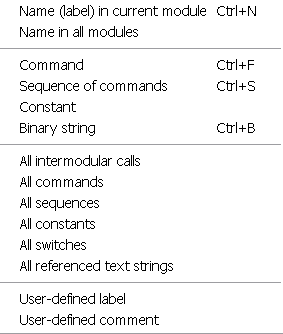
\includegraphics[scale=.40]{images/olly/search.png}
    \end{columns}
\end{frame}

\begin{frame}
    \frametitle{Run Trace and Animate}
    \begin{itemize}
        \item These features are unique to OllyDbg
        \item Animate is useful for watching loop or recursion activity
        \item Run trace is useful for all sorts of tasks
        \begin{itemize}
            \item Unfortunately run trace is extremely slow
            \item Speed was a major motivating factor in my development of alternative code coverage techniques
            \item Pedram can show you demo's of Process Stalker and PaiMei if we have time
        \end{itemize}
    \end{itemize}
\end{frame}
